% This is "sig-alternate.tex" V2.1 April 2013
% This file should be compiled with V2.5 of "sig-alternate.cls" May 2012
%
% This example file demonstrates the use of the 'sig-alternate.cls'
% V2.5 LaTeX2e document class file. It is for those submitting
% articles to ACM Conference Proceedings WHO DO NOT WISH TO
% STRICTLY ADHERE TO THE SIGS (PUBS-BOARD-ENDORSED) STYLE.
% The 'sig-alternate.cls' file will produce a similar-looking,
% albeit, 'tighter' paper resulting in, invariably, fewer pages.
%
% ----------------------------------------------------------------------------------------------------------------
% This .tex file (and associated .cls V2.5) produces:
%       1) The Permission Statement
%       2) The Conference (location) Info information
%       3) The Copyright Line with ACM data
%       4) NO page numbers
%
% as against the acm_proc_article-sp.cls file which
% DOES NOT produce 1) thru' 3) above.
%
% Using 'sig-alternate.cls' you have control, however, from within
% the source .tex file, over both the CopyrightYear
% (defaulted to 200X) and the ACM Copyright Data
% (defaulted to X-XXXXX-XX-X/XX/XX).
% e.g.
% \CopyrightYear{2007} will cause 2007 to appear in the copyright line.
% \crdata{0-12345-67-8/90/12} will cause 0-12345-67-8/90/12 to appear in the copyright line.
%
% ---------------------------------------------------------------------------------------------------------------
% This .tex source is an example which *does* use
% the .bib file (from which the .bbl file % is produced).
% REMEMBER HOWEVER: After having produced the .bbl file,
% and prior to final submission, you *NEED* to 'insert'
% your .bbl file into your source .tex file so as to provide
% ONE 'self-contained' source file.
%
% ================= IF YOU HAVE QUESTIONS =======================
% Questions regarding the SIGS styles, SIGS policies and
% procedures, Conferences etc. should be sent to
% Adrienne Griscti (griscti@acm.org)
%
% Technical questions _only_ to
% Gerald Murray (murray@hq.acm.org)
% ===============================================================
%
% For tracking purposes - this is V2.0 - May 2012

\documentclass{sig-alternate-05-2015}
\usepackage{epstopdf}
\usepackage{braket}
\usepackage{algorithm}
\usepackage{algorithmic}
% Copyright

\setlength{\paperwidth}{8.5in}
\setlength{\paperheight}{11in}
\pdfpagewidth  = \paperwidth
\pdfpageheight = \paperheight

\usepackage{amssymb}
\usepackage{amsmath}
% \usepackage{amsthm}
\interdisplaylinepenalty=2500

% style settings are:
% \clubpenalty=10000
% \widowpenalty=10000

% \setlength{\itemsep}{5pt plus5pt minus0pt} \setlength{\parsep}{5pt
%    plus5pt minus0pt} \setlength{\textfloatsep}{7pt plus0pt
%    minus0pt}%space between graph and text one col
% \setlength{\dbltextfloatsep}{5pt plus5pt
%   minus5pt}% space between graph and tex
% \setlength{\dblfloatsep}{2pt plus0pt minus0pt}%space between graph
% \setlength{\intextsep}{0pt plus0pt minus0pt}%space left on top and

% \usepackage[colorlinks=true, citecolor=blue, urlcolor=cyan, linkcolor=red]{hyperref}


\usepackage{amscd,amsfonts,amsbsy,rotating}
\usepackage{graphicx}
% \usepackage{epsfig,epstopdf}
\usepackage{subfigure}
\usepackage{multirow}
\usepackage{booktabs}
\usepackage{color,xcolor}
\usepackage{url}
\usepackage{latexsym,bm}
\usepackage{enumitem,balance,mathtools}
\usepackage{wrapfig}
\usepackage{mathrsfs,euscript}
\usepackage{algorithm}
\usepackage{algorithmic}
\usepackage{ifpdf}
\usepackage{diagbox}
\usepackage{caption}
\usepackage{makecell}


\newcommand{\bs}{\boldsymbol}
\newcommand{\bx}{\bs{x}}
\newcommand{\btheta}{\bs{\theta}}
\newcommand{\bw}{\mathbf{w}}
\newcommand{\pctr}{r}
\linespread{0.950}

\usepackage{array}
\newcolumntype{N}{@{}m{0pt}@{}}

\newcommand{\waby}[1]{{\bf \color{blue} [[waby says ``#1'']]}}
\newcommand{\qiuchi}[1]{{\bf \color{red} [[qiuchi says ``#1'']]}}
% \newcommand{\jun}[1]{{\bf \color{green} [[Jun says ``#1'']]}}
% \newcommand{\lantao}[1]{{\bf \color{purple} [[Lantao says ``#1'']]}}
% \newcommand{\yu}[1]{{\bf \color{orange} [[Yu says ``#1'']]}}
% \newcommand{\xu}[1]{{\bf \color{violet} [[Yinghui says ``#1'']]}}
% \newcommand{\pz}[1]{{\bf \color{brown} [[Peng says ``#1'']]}}

\renewcommand{\algorithmicrequire}{\textbf{Input:}}  % Use Input in the format of Algorithm
\renewcommand{\algorithmicensure}{\textbf{Output:}} % Use Output in the format of Algorithm

\newcommand{\minisection}[1]{\vspace{5pt}\noindent\textbf{#1.}}
\begin{document}

% Copyright
\setcopyright{acmcopyright}
%\setcopyright{acmlicensed}
%\setcopyright{rightsretained}
%\setcopyright{usgov}
%\setcopyright{usgovmixed}
%\setcopyright{cagov}
%\setcopyright{cagovmixed}


% DOI
\doi{10.475/123_4}

% ISBN
\isbn{123-4567-24-567/08/06}

%Conference
\conferenceinfo{PLDI '13}{June 16--19, 2013, Seattle, WA, USA}

\acmPrice{\$15.00}

%
% --- Author Metadata here ---
\conferenceinfo{WOODSTOCK}{'97 El Paso, Texas USA}
%\CopyrightYear{2007} % Allows default copyright year (20XX) to be over-ridden - IF NEED BE.
%\crdata{0-12345-67-8/90/01}  % Allows default copyright data (0-89791-88-6/97/05) to be over-ridden - IF NEED BE.
% --- End of Author Metadata ---

\title{Quantum Memory Network for Language Modelling
%\titlenote{(Produces the permission block, and copyright information). For use with SIG-ALTERNATE.CLS. Supported by ACM.}
}
% \subtitle{[Extended Abstract]
% \titlenote{A full version of this paper is available as
% \textit{Author's Guide to Preparing ACM SIG Proceedings Using
% \LaTeX$2_\epsilon$\ and BibTeX} at
% \texttt{www.acm.org/eaddress.htm}}}
%
% You need the command \numberofauthors to handle the 'placement
% and alignment' of the authors beneath the title.
%
% For aesthetic reasons, we recommend 'three authors at a time'
% i.e. three 'name/affiliation blocks' be placed beneath the title.
%
% NOTE: You are NOT restricted in how many 'rows' of
% "name/affiliations" may appear. We just ask that you restrict
% the number of 'columns' to three.
%
% Because of the available 'opening page real-estate'
% we ask you to refrain from putting more than six authors
% (two rows with three columns) beneath the article title.
% More than six makes the first-page appear very cluttered indeed.
%
% Use the \alignauthor commands to handle the names
% and affiliations for an 'aesthetic maximum' of six authors.
% Add names, affiliations, addresses for
% the seventh etc. author(s) as the argument for the
% \additionalauthors command.
% These 'additional authors' will be output/set for you
% without further effort on your part as the last section in
% the body of your article BEFORE References or any Appendices.

% \numberofauthors{8} %  in this sample file, there are a *total*
% % of EIGHT authors. SIX appear on the 'first-page' (for formatting
% % reasons) and the remaining two appear in the \additionalauthors section.
% %
% \author{
% % You can go ahead and credit any number of authors here,
% % e.g. one 'row of three' or two rows (consisting of one row of three
% % and a second row of one, two or three).
% %
% % The command \alignauthor (no curly braces needed) should
% % precede each author name, affiliation/snail-mail address and
% % e-mail address. Additionally, tag each line of
% % affiliation/address with \affaddr, and tag the
% % e-mail address with \email.
% %
% % 1st. author
% \alignauthor
% Ben Trovato\titlenote{Dr.~Trovato insisted his name be first.}\\
%        \affaddr{Institute for Clarity in Documentation}\\
%        \affaddr{1932 Wallamaloo Lane}\\
%        \affaddr{Wallamaloo, New Zealand}\\
%        \email{trovato@corporation.com}
% % 2nd. author
% \alignauthor
% G.K.M. Tobin\titlenote{The secretary disavows
% any knowledge of this author's actions.}\\
%        \affaddr{Institute for Clarity in Documentation}\\
%        \affaddr{P.O. Box 1212}\\
%        \affaddr{Dublin, Ohio 43017-6221}\\
%        \email{webmaster@marysville-ohio.com}
% % 3rd. author
% \alignauthor Lars Th{\o}rv{\"a}ld\titlenote{This author is the
% one who did all the really hard work.}\\
%        \affaddr{The Th{\o}rv{\"a}ld Group}\\
%        \affaddr{1 Th{\o}rv{\"a}ld Circle}\\
%        \affaddr{Hekla, Iceland}\\
%        \email{larst@affiliation.org}
% \and  % use '\and' if you need 'another row' of author names
% % 4th. author
% \alignauthor Lawrence P. Leipuner\\
%        \affaddr{Brookhaven Laboratories}\\
%        \affaddr{Brookhaven National Lab}\\
%        \affaddr{P.O. Box 5000}\\
%        \email{lleipuner@researchlabs.org}
% % 5th. author
% \alignauthor Sean Fogarty\\
%        \affaddr{NASA Ames Research Center}\\
%        \affaddr{Moffett Field}\\
%        \affaddr{California 94035}\\
%        \email{fogartys@amesres.org}
% % 6th. author
% \alignauthor Charles Palmer\\
%        \affaddr{Palmer Research Laboratories}\\
%        \affaddr{8600 Datapoint Drive}\\
%        \affaddr{San Antonio, Texas 78229}\\
%        \email{cpalmer@prl.com}
% }
% % There's nothing stopping you putting the seventh, eighth, etc.
% % author on the opening page (as the 'third row') but we ask,
% % for aesthetic reasons that you place these 'additional authors'
% % in the \additional authors block, viz.
% \additionalauthors{Additional authors: John Smith (The Th{\o}rv{\"a}ld Group,
% email: {\texttt{jsmith@affiliation.org}}) and Julius P.~Kumquat
% (The Kumquat Consortium, email: {\texttt{jpkumquat@consortium.net}}).}
% \date{30 July 1999}
% % Just remember to make sure that the TOTAL number of authors
% % is the number that will appear on the first page PLUS the
% % number that will appear in the \additionalauthors section.

\maketitle
\begin{abstract}

Sequential modelling is one of the key concern in textual represention. Recurrent Neural Network is a typicial practice for the textual task with sequential order. However, the hidden state of RNN and its variants  lack some interpretability for  human, which is called a black box. In this paper, we propose a new approach, namely Quantum Memory Network (QMN), to model a real-time semantic state in a dynamic sequential progress. Inspired by the quantum measurement, such semantic state is designed to descibe a explict distribution over all the semantic space via quantum density martix. The experiments \footnote{https://github.com/wabyking/QuantumMemoryNetwork} demostrate our model significantly outperform the baseline model. 



\end{abstract}


%
% The code below should be generated by the tool at
% http://dl.acm.org/ccs.cfm
% Please copy and paste the code instead of the example below. 
%
\begin{CCSXML}
<ccs2012>
 <concept>
  <concept_id>10010520.10010553.10010562</concept_id>
  <concept_desc>Computer systems organization~Embedded systems</concept_desc>
  <concept_significance>500</concept_significance>
 </concept>
 <concept>
  <concept_id>10010520.10010575.10010755</concept_id>
  <concept_desc>Computer systems organization~Redundancy</concept_desc>
  <concept_significance>300</concept_significance>
 </concept>
 <concept>
  <concept_id>10010520.10010553.10010554</concept_id>
  <concept_desc>Computer systems organization~Robotics</concept_desc>
  <concept_significance>100</concept_significance>
 </concept>
 <concept>
  <concept_id>10003033.10003083.10003095</concept_id>
  <concept_desc>Networks~Network reliability</concept_desc>
  <concept_significance>100</concept_significance>
 </concept>
</ccs2012>  
\end{CCSXML}

\ccsdesc[500]{Computer systems organization~Embedded systems}
\ccsdesc[300]{Computer systems organization~Redundancy}
\ccsdesc{Computer systems organization~Robotics}
\ccsdesc[100]{Networks~Network reliability}


%
% End generated code
%

%
%  Use this command to print the description
%
\printccsdesc

% We no longer use \terms command
%\terms{Theory}

\keywords{ACM proceedings; \LaTeX; text tagging}

\section{Introduction}


Sequential language modeling is a one of key concerns in Textual Information Retrieval and Natural Language Processing. Current state of art models like Recurrent Neural Network and it variants (LSTM and further) use a black-box  mechanism to model language, which easily achieve  a better performance in the current supervised dataset, but lack some inherent interpretability thus can not generate its similar conclusion to another dataset. Limited efforts  are trying to explain the inner mechanism in sequential neural network (e.g. RNN, Encoder-Decoder, Memory Network), but in an empirical post-hoc conjecture after training \cite{lipton2016mythos}, e.g. network visualizing in neural machine translation \cite{ding2017visualizing},  clustering analyzing for word embeddings \cite{trost2017parameter} and understanding hidden state vectors in neural readers\cite{wang2017emergent}. Interpretability in the perspective of transparency tends to be a vital issue for us to understand the mechanism by how these models work.  \cite{levine2017deep} uses tensor networks and tensor decompositions to bridge the gap between conventional neural network, which opens a new door for us to use quantum-inspired insight to motivate us to design new self-explanatory neural networks.

Recently, Quantum Theory have been applied into many fields outside of physics, e.g. Information Retrieval\cite{van2004geometry,melucci2011quantum}, Natural Language Processing\cite{blacoe2013quantum,zhang2018end}. In the language representation and matching task, Quantum and Quantum-inspired models are firstly introduced in ad hoc retrieval. These works \cite{zuccon2010using} usually design some Quantum inspired approach to rank documents, intrinsically, the representation of document/language is still based on traditional IR models. 
Many works \cite{piwowarski2010can,sordoni2013modeling1} are trying to model  document (query) in quantum representation (e.g. density matrix and subspace). However, they are usually based on bag-of-word models for ad-hoc retrieval, which is limited to model a sequential textual sentence.  \cite{zhang2018end} propose a end-2-end neural network to calculate the question-answer matching score via convolution over the inner product of question and answer density matrices, but it is totally designed in traditional neural network but  have little quantum property within the models.

\begin{figure}[h]
\centering
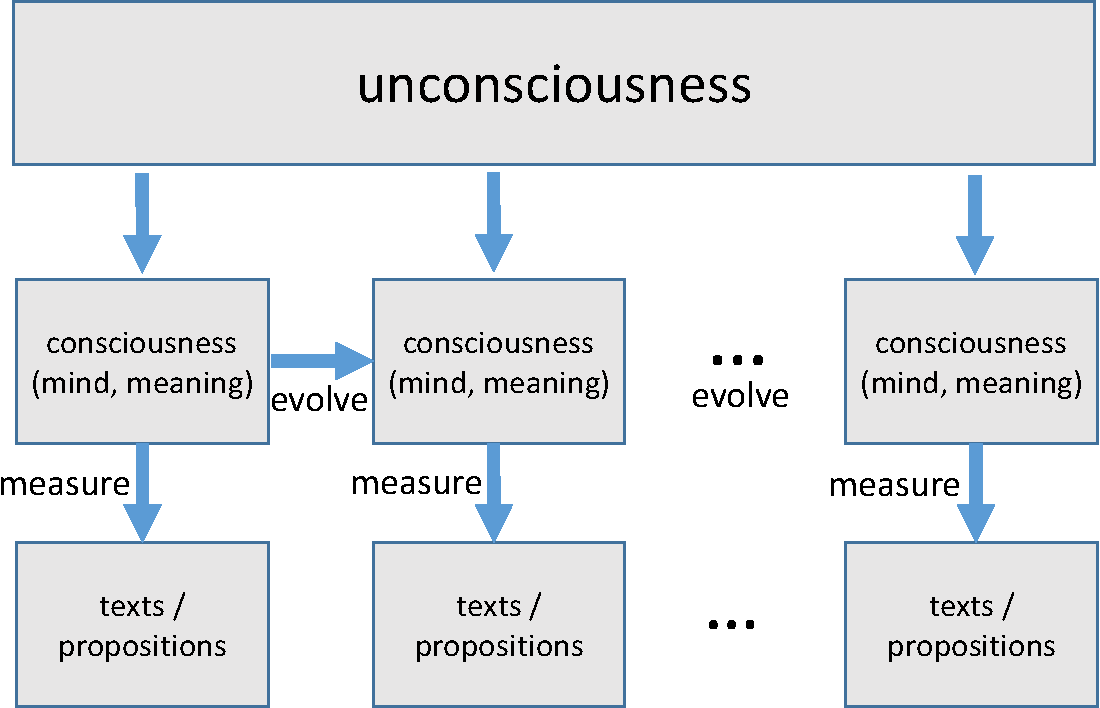
\includegraphics[ width=3in]{figures/measurement-crop.pdf}
\caption{The process of measurement for a sequential sentence}
\label{fig:measurement}
%\vspace{-10pt}
\end{figure}
Most of the above quantum models propose a series of static representation for a sentence or a document, which is too rough to model the complexity of language. Language could be considered a dynamic process derived from our mind in a cognitive perspective \cite{atmanspacher2012dual}. we develop the idea from \cite{xie2015modeling} in a dynamic evolution settings, as illustrated in Figure \ref{fig:measurement}. \cite{atmanspacher2012dual} propose that  the unconscious state  can be seen as an entangled state, and then becoming  a conscious state after measurement. \cite{xie2015modeling} further explain that the process from consciousness to a static word sequence in only one measurement. In our deeper thinking, the consciousness collapses to a word or a phrase after each measurement, as seem for us in reality. In the same time, the consciousness can also be affected and instantly transfered into a new state, and can also collapses to a new word or  phrase in a dynamic process. 

In our paper, we design a Quantum Memory Network to model the dynamic process from consciousness to a sequence of words/phrases. Each word/phrase are denoted as a N-dimensional unit vector in a Hibert space, while consciousness is denoted as density matrix. After a measurement, the  state of consciousness will  in principle (completely or slightly) collapse, thus becoming to a new state.  In a specific context (with many measured words before), the state of consciousness can be described as a semantic distribution over all the words. Such distribution would be affected by each measuring result, namely, would evolve with the word generating.

The experimental result \footnote{https://github.com/wabyking/QuantumMemoryNetwork } demonstrate the advantage of our models in some typical task, like ,word regulation, word similarity, language model, Sentence Classification,  Microsoft Research Paraphrase Corpus (Dolan and Brockett 200),  Semantic Similarity (SICK Dataset (Marelli et al. 2014)), Textual Entailment(Stanford Natural Language Inference Dataset (Bowman et al. 2015)), Question answering and ad hoc Retrieval.





\section{Related Works}
\subsection{Quantum Information Retrieval}
\subsection{Recurrent Neural Network and Memory Network}
\subsection{Markov Decision Process}
\section{Quantum Preliminaries}
\section{Models}
\subsection{Representation}
\subsubsection{Unit word vector}
\subsubsection{Density Matrix}
povm exmplain
\subsection{Evolution}


\begin{equation}
\alpha = \braket{h|e_{w_i}}^2
\label{eq:bias}
\end{equation}

\begin{equation}
\rho^{(t)} = \rho^{(t-1)} * \alpha + \ket{e_{w_i}}\bra{e_{w_i}} *(1-\alpha)
\label{eq:update}
\end{equation}

\begin{equation}
loss = distance(softmax(\rho^{(t)}*E), Onehot(w_(i+1)))
\label{eq:loss}
\end{equation}


\begin{algorithm}[t]
\caption{Training of Quantum Memory Network}
\label{algo:framework}
\begin{algorithmic}[1]
\small
\REQUIRE
m-dimension word vectors $E$ with size $|V|*m$ \\
\hspace{4mm} A assisted hidden vector $h$ for measurement   \\
\hspace{4mm} A given word sequence $\mathcal{S}=\left\{\bs{w_1},\bs{w_2},...\bs{w_n}\right\}$ \\
\hspace{4mm} A initial density matrix $\rho _0$   \\

\STATE
Initialise $\rho=\rho _0$.
\STATE
Pretrain  embedding and grantee the unit length.

\REPEAT
\FOR{ i : n}
\STATE
Look up the unit word vector $e_{w_i}$ for word $w_i$.
\STATE
Calculate the bias of the weak measurement by Eq.~({\ref{eq:bias}}).
\STATE
Update the new density matrix  by Eq.~({\ref{eq:update}}).
\STATE
Back propagation by loss shown in  Eq.~({\ref{eq:loss}}).
\ENDFOR

\UNTIL{Traversal all the tokens in current sentence.}
\end{algorithmic}
\end{algorithm}


\subsection{Optimization Method}

\section{Empirical Evaluation}
\subsection{Dataset}
\subsection{Metric}
\subsection{Result and Analysis}
\subsection{Ablation test}
\subsection{Parameter Sensitivity}
\section{Discussion}
\subsection{Time Complexity}
\subsection{Space Complexity}
\subsection{Case Study}
\section{Conclusions}
This paragraph will end the body of this sample document.
Remember that you might still have Acknowledgments or
Appendices; brief samples of these
follow.  There is still the Bibliography to deal with; and
we will make a disclaimer about that here: with the exception
of the reference to the \LaTeX\ book, the citations in
this paper are to articles which have nothing to
do with the present subject and are used as
examples only.
%\end{document}  % This is where a 'short' article might terminate

%ACKNOWLEDGMENTS are optional
\section{Acknowledgments}
This section is optional; it is a location for you
to acknowledge grants, funding, editing assistance and
what have you.  In the present case, for example, the
authors would like to thank Gerald Murray of ACM for
his help in codifying this \textit{Author's Guide}
and the \textbf{.cls} and \textbf{.tex} files that it describes.

%
% The following two commands are all you need in the
% initial runs of your .tex file to
% produce the bibliography for the citations in your paper.
\bibliographystyle{abbrv}
\bibliography{sigproc}  % sigproc.bib is the name of the Bibliography in this case
% You must have a proper ".bib" file
%  and remember to run:
% latex bibtex latex latex
% to resolve all references
%
% ACM needs 'a single self-contained file'!
%
%APPENDICES are optional
%\balancecolumns
\appendix
%Appendix A
\section{Regarding Density Matrix}
Understand Density Matrix.
\section{Standard Measurement and Weak Measurement}
Why we do not use Standard Measurement 
\end{document}
